\section{Modello di Sviluppo}
\label{ModelloSviluppo}

Dopo un'attenta analisi dei vari modelli di sviluppo, abbiamo  scelto di utilizzare il modello di tipo incrementale.

\subsection{Modello Incrementale}

\begin{figure}[h]
	\centering
  		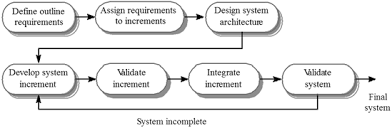
\includegraphics[width=0.7\linewidth]{./images/modelloincrementale.png}
  		\caption{Modello Incrementale da : \url{https://www.math.unipd.it/~tullio/IS-1/2015/Dispense/L03.pdf} slide numero 18}
  		\label{fig:Modello Incrementale}
\end{figure}

Il modello incrementale prevede rilasci multipli e successivi del prodotto ed ogni rilascio prevede un incremento delle sue funzionalità. \\
Con questo modello vengono pianificati quanti incrementi verranno effettuati basandosi sui requisiti obbligatori ed opzionali richiesti dalla proponente, aggiungendovi delle priorità di sviluppo in modo tale che elementi con priorità maggiore vengano sviluppati prima di elementi con priorità minore.\\
Il prodotto finale non sarà rilasciato nella sua completezza in un solo momento ma prevederà, appunto, degli incrementi. \\
È fondamentale decidere i requisiti con completezza prima di iniziare lo sviluppo dell'attuale incremento, mentre requisiti aggiuntivi per incrementi futuri sono adeguati. Per ogni sviluppo delle parti è necessario analizzare il suo grado di efficacia\glossario prima di integrare le parti tra di loro. Terminato l'incremento attuale si andrà avanti con l'incremento successivo scelto precedentemente, qualora il prodotto non sia completo. \\
Il vantaggio di utilizzare questo modello racchiude, tra le varie, un rilascio delle funzionalità base nei primi incrementi, il che comporta una maggiore verifica e quindi una maggiore stabilità. Oltretutto i primi incrementi possono derivare da una prototipazione, la quale aiuta a fissare meglio i requisiti per gli elementi successivi. Un ulteriore vantaggio è la riduzione del rischio di fallimento, senza azzerarlo in quanto costi aggiuntivi posso derivare dalla caduta nell'iterazione\glossario.

\subsubsection{Incremento}
\label{inc}

La durata di un incremento è di dieci giorni ed è composto dalle seguenti fasi:
\begin{itemize}
	\item Assegnazione dei task ai componenti del gruppo il primo giorno;
	\item Completamento dei task dal secondo all'ottavo giorno;
	\item Verifica e valutazione del prodotto nei giorni rimanenti.
\end{itemize}

In questo modo il numero di incrementi è superiormente limitato in decadi, e dovranno rispettare i periodi descritti nel capitolo seguente.  